\chapter{Techniques de laboratoire, I~: sécurité, mesure et séparation}\label{ch:b1:lab-techniques-1}

Deux étudiants recristallisent le même lot d'aspirine et mesurent sa
température de fusion sur le même banc chauffant. L'un lit
\qty{134}{\celsius}, l'autre \qty{136}{\celsius}. Sont-ils en
désaccord~? Le produit est-il pur~? Aucune de ces questions ne peut être
tranchée à partir des deux nombres seuls~: une mesure ne vaut que par son
incertitude, et une comparaison que par une règle. Ce dernier chapitre
rassemble le versant pratique de l'année~: comment lire les \omterm{def:b1:lab-techniques-1:hazard}{dangers} de
ce qui se trouve sur la paillasse, comment énoncer une valeur mesurée et
son incertitude et la comparer à une autre, et comment les opérations
classiques du laboratoire de chimie organique --- extraction, filtration,
\omterm{def:b1:lab-techniques-1:recrystallisation}{recristallisation}, distillation --- séparent un produit de ce qui
l'entoure, puis vérifient qu'il est pur.

\begin{recall}
La \omterm{def:b1:precipitation:solubility}{solubilité} et la miscibilité expliquées par les interactions
intermoléculaires, les \omterm{def:b1:intermolecular-forces-solvents:solvent-classes}{solvants polaires} et apolaires
(\cref{ch:b1:intermolecular-forces-solvents})~; les burettes, les
pipettes et le point de fin d'un \omterm{def:b1:titration-methods:titration}{titrage} (\cref{ch:b1:titration-methods}).
Le volume scolaire (année 10) a introduit l'extraction liquide--liquide,
la \omterm{def:b1:lab-techniques-1:recrystallisation}{recristallisation}, la chromatographie sur couche mince et le
\omterm{def:b1:extent-q-and-k:fractional-extent}{rendement} d'une synthèse~; ils reçoivent ici leurs nombres.
\end{recall}

\begin{omfigure}
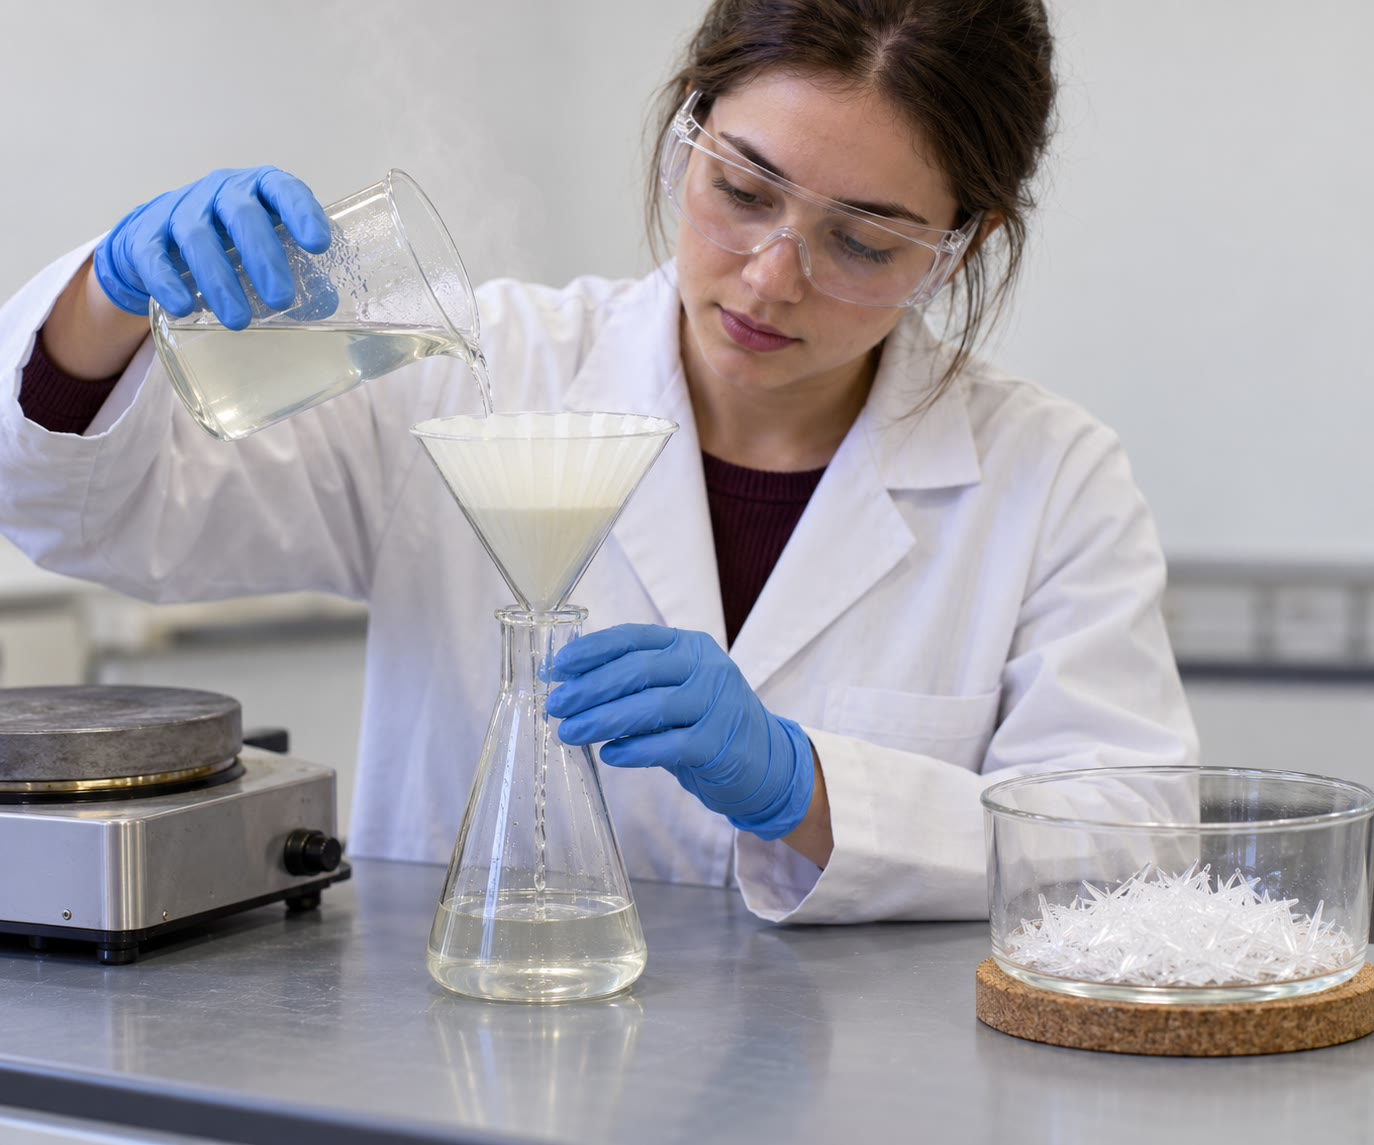
\includegraphics[width=0.5\linewidth]{images/book2/ai/b1-29-recrystallisation.jpg}

{\small Filtration à chaud lors d'une \omterm{def:b1:lab-techniques-1:recrystallisation}{recristallisation}~: lunettes, gants
et blouse~; la solution chaude traverse un papier filtre plissé, qui
retient les impuretés insolubles. Des aiguilles d'un produit
recristallisé attendent dans la coupelle de droite.}
\end{omfigure}

\section{Les dangers et leur étiquetage}

\begin{definition}[Danger et risque]\label{def:b1:lab-techniques-1:hazard}
Un \emph{danger}\index{danger} est la propriété intrinsèque d'une
substance (ou d'une situation) susceptible de causer un dommage~:
inflammabilité, corrosivité, toxicité. Le \emph{risque}\index{risque}
est la probabilité que le dommage survienne effectivement, et sa
gravité, dans les conditions d'utilisation données~: il dépend du
danger et de l'exposition (quantité, concentration, durée, voie
d'exposition, protection).
\end{definition}

On ne peut pas changer un \omterm{def:b1:lab-techniques-1:hazard}{danger} sans changer la substance~; on réduit un
\omterm{def:b1:lab-techniques-1:hazard}{risque} en agissant sur l'exposition~: une quantité plus petite, une
solution plus diluée, une hotte, des gants et des lunettes, ou un réactif
moins dangereux pour le même usage.

\begin{definition}[Étiquetage SGH]\label{def:b1:lab-techniques-1:ghs}
L'étiquetage des produits chimiques suit le Système général harmonisé
(SGH, en anglais GHS).
\begin{itemize}
  \item Un \emph{pictogramme de danger}\index{pictogramme de danger} est
        un symbole noir sur un losange blanc bordé de rouge~; il y en a
        neuf, de \texttt{GHS01} à \texttt{GHS09}.
  \item La \emph{mention d'avertissement}\index{mention d'avertissement}
        est \emph{Danger} pour les catégories de \omterm{def:b1:lab-techniques-1:hazard}{danger} les plus graves et
        \emph{Attention} pour les moins graves~; une étiquette n'en porte
        qu'une, la plus grave.
  \item Une \emph{mention de danger}\index{mention de danger} est une
        phrase normalisée, codée H suivi de trois chiffres, qui décrit un
        \omterm{def:b1:lab-techniques-1:hazard}{danger}~: H2xx \omterm{def:b1:lab-techniques-1:hazard}{dangers} physiques, H3xx \omterm{def:b1:lab-techniques-1:hazard}{dangers} pour la santé, H4xx
        \omterm{def:b1:lab-techniques-1:hazard}{dangers} pour l'environnement.
  \item Un \emph{conseil de prudence}\index{conseil de prudence}, codé P
        et trois chiffres, indique une mesure à prendre~: P1xx généralités,
        P2xx prévention, P3xx intervention, P4xx stockage, P5xx
        élimination.
  \item La \emph{fiche de données de sécurité}\index{fiche de donnees de securite@fiche de données de sécurité}
        est le document que le fournisseur remet avec un produit, en
        rubriques normalisées~: identification, \omterm{def:b1:lab-techniques-1:hazard}{dangers}, composition,
        premiers secours, lutte contre l'incendie, manipulation et
        stockage, contrôle de l'exposition et protection individuelle,
        propriétés physiques et chimiques, stabilité, toxicité,
        élimination et transport.
\end{itemize}
\end{definition}

\begin{omfigure}
\setlength{\tabcolsep}{5pt}
\begin{tabular}{ccccc}
\begin{tabular}[t]{@{}c@{}}\ghs[1.25cm]{GHS01}\\[2pt]\footnotesize GHS01\\\footnotesize explosif\end{tabular} &
\begin{tabular}[t]{@{}c@{}}\ghs[1.25cm]{GHS02}\\[2pt]\footnotesize GHS02\\\footnotesize inflammable\end{tabular} &
\begin{tabular}[t]{@{}c@{}}\ghs[1.25cm]{GHS03}\\[2pt]\footnotesize GHS03\\\footnotesize comburant\end{tabular} &
\begin{tabular}[t]{@{}c@{}}\ghs[1.25cm]{GHS04}\\[2pt]\footnotesize GHS04\\\footnotesize gaz sous pression\end{tabular} &
\begin{tabular}[t]{@{}c@{}}\ghs[1.25cm]{GHS05}\\[2pt]\footnotesize GHS05\\\footnotesize corrosif\end{tabular} \\[8pt]
\begin{tabular}[t]{@{}c@{}}\ghs[1.25cm]{GHS06}\\[2pt]\footnotesize GHS06\\\footnotesize toxicité aiguë\end{tabular} &
\begin{tabular}[t]{@{}c@{}}\ghs[1.25cm]{GHS07}\\[2pt]\footnotesize GHS07\\\footnotesize nocif, irritant\end{tabular} &
\begin{tabular}[t]{@{}c@{}}\ghs[1.25cm]{GHS08}\\[2pt]\footnotesize GHS08\\\footnotesize danger pour la santé\end{tabular} &
\begin{tabular}[t]{@{}c@{}}\ghs[1.25cm]{GHS09}\\[2pt]\footnotesize GHS09\\\footnotesize environnement\end{tabular} & \\
\end{tabular}

\smallskip
{\small Les neuf pictogrammes du SGH~: bombe explosant, flamme, flamme
au-dessus d'un cercle, bouteille de gaz, corrosion, tête de mort sur
tibias croisés, point d'exclamation, danger pour la santé (effets à long
terme~: cancer, mutations, reproduction, sensibilisation des voies
respiratoires, toxicité par aspiration) et environnement.}
% ledger: ghspic:GHS01, ghspic:GHS02, ghspic:GHS03, ghspic:GHS04,
% ghspic:GHS05, ghspic:GHS06, ghspic:GHS07, ghspic:GHS08, ghspic:GHS09
\end{omfigure}

\begin{example}[Lire l'étiquette de l'éthanol]
Un flacon d'éthanol porte les pictogrammes GHS02 et GHS07, la \omterm{def:b1:lab-techniques-1:ghs}{mention
d'avertissement} \emph{Danger}, et les mentions H225 (liquide et vapeurs
très inflammables, un \omterm{def:b1:lab-techniques-1:hazard}{danger} physique dont la catégorie impose
\emph{Danger}) et H319 (provoque une sévère irritation des yeux, un
danger pour la santé, qui n'appellerait à lui seul que
\emph{Attention}). Ses \omterm{def:b1:lab-techniques-1:ghs}{conseils de prudence} comprennent P210 (tenir à
l'écart de la chaleur, des étincelles et des flammes nues~; ne pas
fumer), P233 (maintenir le récipient fermé de manière étanche), P280
(porter des gants et une protection des yeux), P305+P351+P338 (en cas de
contact avec les yeux~: rincer avec précaution à l'eau pendant plusieurs
minutes, enlever les lentilles de contact, continuer à rincer) et
P403+P235 (stocker dans un endroit bien ventilé, tenir au frais). Les
conséquences pratiques~: aucune flamme sur la paillasse où l'on utilise
l'éthanol, des lunettes, un flacon fermé.
\end{example}
% ledger: ghs:ethanol, hstat:H225, hstat:H319, pstat:P210, pstat:P233,
% pstat:P280, pstat:P305+P351+P338, pstat:P403+P235

\begin{method}[Préparer une séance à partir des fiches de données de sécurité]\label{met:b1:lab-techniques-1:read-sds}
Pour chaque substance utilisée ou formée~:
\begin{enumerate}
  \item lire ses pictogrammes, sa \omterm{def:b1:lab-techniques-1:ghs}{mention d'avertissement} et ses mentions
        H (rubrique 2 de la fiche), et relever les \omterm{def:b1:lab-techniques-1:hazard}{dangers} physiques
        (incendie, pression, réactivité) à part des \omterm{def:b1:lab-techniques-1:hazard}{dangers} pour la santé
        et pour l'environnement~;
  \item pour chaque opération (pesée, chauffage, transvasement,
        filtration), estimer l'exposition~: quantité, état (un liquide
        volatil ou une poudre fine atteint les poumons), durée~;
  \item choisir les mesures~: substitution par un réactif moins
        dangereux, échelle réduite, hotte, puis protection individuelle
        (conseils P2xx)~;
  \item prévoir la conduite à tenir en cas d'incident (P3xx~: yeux, peau,
        ingestion, incendie) et la destination de chaque déchet (P5xx).
\end{enumerate}
\end{method}

\begin{inthelab}[Les déchets]
Rien ne part à l'évier par défaut. Les solvants organiques sont collectés
dans deux bidons, halogénés (dichlorométhane, chloroforme) et non
halogénés (éthanol, propanone, cyclohexane, éthanoate d'éthyle), car ils
sont traités différemment~; les solutions aqueuses acides et basiques
sont neutralisées avant élimination~; les solutions d'ions de métaux
lourds (chrome, cuivre, argent) ont leurs propres bidons~; le verre
cassé et les solides contaminés sont tenus à l'écart des ordures
ordinaires. Le conseil P273, «~éviter le rejet dans
l'environnement~», sur une étiquette, rappelle que c'est le bidon de
récupération, et non l'égout, qui marque la fin de l'expérience.
% ledger: pstat:P273
\end{inthelab}

\section{Mesure et incertitude}

Une valeur mesurée n'est jamais la valeur exacte de la grandeur
mesurée~: répétez la mesure, et le résultat change un peu~; lisez la
graduation, et le dernier chiffre est une estimation. L'incertitude
indique à quelle distance de la valeur mesurée la valeur vraie peut
raisonnablement se trouver.

\begin{definition}[Incertitude de mesure]\label{def:b1:lab-techniques-1:uncertainty}
\begin{itemize}
  \item L'\emph{incertitude de mesure}\index{incertitude de mesure} est
        un paramètre qui caractérise la dispersion des valeurs que l'on
        peut raisonnablement attribuer à la grandeur mesurée.
  \item L'\emph{incertitude-type}\index{incertitude-type} $u(x)$ est
        cette incertitude exprimée sous la forme d'un écart-type.
  \item Une \emph{évaluation de type A}\index{evaluation de type A@évaluation de type A}
        obtient $u$ par
        l'analyse statistique d'une série de mesures répétées~; une
        \emph{évaluation de type B}\index{evaluation de type B@évaluation de type B}
        l'obtient par tout autre moyen~: la graduation d'un instrument, la
        tolérance indiquée par son fabricant, un certificat d'étalonnage,
        le nombre de chiffres d'une valeur tabulée.
  \item L'\emph{incertitude élargie}\index{incertitude elargie@incertitude élargie}
        $U = k\,u$ est l'incertitude-type multipliée par un facteur
        d'élargissement $k$, en général $k = 2$~; pour une distribution
        normale, l'intervalle $x \pm 2u$ contient la valeur vraie avec une
        probabilité d'environ \qty{95}{\percent}.
  \item L'\emph{incertitude relative}\index{incertitude relative} est
        $u(x)/|x|$, souvent exprimée en pourcentage.
\end{itemize}
\end{definition}

\begin{proposition}[Évaluation de type A]\label{prop:b1:lab-techniques-1:type-a}
Si l'on effectue $n$ mesures indépendantes $x_1, \dots, x_n$ d'une même
grandeur, la meilleure estimation est leur moyenne $\bar x$~;
l'écart-type expérimental vaut
\[
  s = \sqrt{\frac{1}{n-1} \sum_{i=1}^{n} (x_i - \bar x)^2},
\]
et l'\omterm{def:b1:lab-techniques-1:uncertainty}{incertitude-type} de la moyenne vaut $u(\bar x) = s/\sqrt{n}$.
\end{proposition}
\begin{proof}[\omnameProof]
\emph{Admis à ce niveau}~; la statistique des mesures répétées, y
compris le coefficient de Student utilisé lorsque $n$ est petit, est
traitée dans le volume de deuxième année.
\end{proof}

\begin{omfigure}
\begin{tikzpicture}
\begin{axis}[width=7.4cm, height=5cm, xlabel={volume à l'équivalence (\unit{mL})},
  ylabel={nombre de lectures}, ymin=0, ymax=8.5, xmin=12.2, xmax=12.7,
  xtick={12.2,12.3,12.4,12.5,12.6,12.7},
  xticklabel style={/pgf/number format/fixed, /pgf/number format/precision=1},
  axis lines=left, every axis plot/.append style={line join=round}]
  \addplot[ybar, bar width=0.045, fill=omDef!35, draw=omDef!80!black]
    table[x=V, y=count] {figdata/out/bachelor-1-type-a-uncertainty-a.dat};
  \addplot[omThm, thick, smooth]
    table[x=V, y=g] {figdata/out/bachelor-1-type-a-uncertainty-b.dat};
  \draw[omProp, thick, <->] (axis cs:12.384,7.6) -- (axis cs:12.526,7.6);
  \node[omProp, font=\small, above] at (axis cs:12.455,7.6) {$\bar V \pm s$};
\end{axis}
\end{tikzpicture}\hspace{0.6cm}%
\begin{tikzpicture}
\begin{axis}[width=5.6cm, height=5cm, xlabel={$x - x_0$}, ylabel={densité},
  ymin=0, ymax=0.8, xmin=-1.6, xmax=1.6, xtick={-1,0,1},
  xticklabels={$-a$, $0$, $a$}, ytick={0.5}, yticklabels={$\frac{1}{2a}$},
  axis lines=left]
  \addplot[omDef!80!black, thick, fill=omDef!25] coordinates
    {(-1,0) (-1,0.5) (1,0.5) (1,0)} \closedcycle;
  \draw[omProp, thick, <->] (axis cs:-0.577,0.62) -- (axis cs:0.577,0.62);
  \node[omProp, font=\small, above] at (axis cs:0,0.62) {$\pm a/\sqrt3$};
\end{axis}
\end{tikzpicture}

{\small À gauche~: vingt lectures d'un même \omterm{def:b1:titration-methods:titration}{point de fin de titrage}
(données illustratives), lues à \qty{0.05}{mL} près, avec la courbe
normale de même moyenne
$\bar V = \qty{12.455}{mL}$ et de même écart-type $s = \qty{0.071}{mL}$.
À droite~: la distribution rectangulaire d'une \omterm{def:b1:lab-techniques-1:uncertainty}{évaluation de type B},
pour une valeur dont on sait seulement qu'elle est comprise entre
$x_0 - a$ et $x_0 + a$~; son écart-type vaut
$a/\sqrt3$.}
\end{omfigure}

\begin{example}[Vingt points de fin de titrage]
Pour les vingt lectures de la figure, $\bar V = \qty{12.455}{mL}$,
$s = \qty{0.071}{mL}$ et $u(\bar V) = 0.071/\sqrt{20} = \qty{0.016}{mL}$.
Une lecture est incertaine d'environ $s$~; la moyenne de vingt lectures,
d'environ
$s/\sqrt{20}$, soit quatre fois et demie moins. Le résultat s'écrit
$V = \qty{12.46}{mL}$ avec $U = 2u = \qty{0.03}{mL}$.
\end{example}

\begin{proposition}[Évaluation de type B pour une distribution rectangulaire]\label{prop:b1:lab-techniques-1:type-b}
Si tout ce que l'on sait d'une grandeur est qu'elle se trouve, avec une
probabilité uniforme, n'importe où entre $x_0 - a$ et $x_0 + a$, son
\omterm{def:b1:lab-techniques-1:uncertainty}{incertitude-type} vaut
\[
  u = \frac{a}{\sqrt3}.
\]
\end{proposition}
\begin{proof}
La densité de probabilité vaut $1/(2a)$ sur $[x_0 - a, x_0 + a]$ et zéro
ailleurs~; sa moyenne est $x_0$ par symétrie et sa variance vaut
\[
  u^2 = \int_{x_0-a}^{x_0+a} (x - x_0)^2 \frac{\mathrm{d}x}{2a}
      = \frac{1}{2a} \left[\frac{t^3}{3}\right]_{-a}^{a}
      = \frac{1}{2a}\cdot\frac{2a^3}{3} = \frac{a^2}{3}. \qedhere
\]
\end{proof}

\begin{example}[Une lecture et une tolérance]
Une burette graduée tous les \qty{0.1}{mL} se lit à une demi-graduation
près~: la lecture se trouve à $\pm\qty{0.05}{mL}$ de la valeur notée,
donc
$u = 0.05/\sqrt3 = \qty{0.029}{mL}$. Une pipette de \qty{20}{mL} dont le
fabricant indique une tolérance de $\pm\qty{0.03}{mL}$ délivre son
volume avec
$u = 0.03/\sqrt3 = \qty{0.017}{mL}$. Une valeur tabulée donnée comme
\qty{135}{\celsius} est connue à $\pm\qty{0.5}{\celsius}$ près~: $u = \qty{0.29}{\celsius}$.
\end{example}

\begin{proposition}[Composition des incertitudes]\label{prop:b1:lab-techniques-1:combine}
Pour des grandeurs indépendantes~: si $y = x_1 + x_2$ ou $y = x_1 - x_2$, alors
$u(y)^2 = u(x_1)^2 + u(x_2)^2$~; si $y = x_1 x_2$ ou $y = x_1/x_2$, alors
\[
  \left(\frac{u(y)}{y}\right)^2 = \left(\frac{u(x_1)}{x_1}\right)^2
  + \left(\frac{u(x_2)}{x_2}\right)^2 .
\]
Plusieurs sources d'incertitude portant sur une même grandeur (une part
de type A et des parts de type B) se composent de la même façon, en
somme de carrés.
\end{proposition}
\admitted

Ce sont les carrés, et non les incertitudes elles-mêmes, qui
s'additionnent~: deux erreurs indépendantes poussent rarement dans le
même sens avec toute leur ampleur. Un volume titré est la différence de
deux lectures de burette, si bien que son incertitude de lecture vaut
$\sqrt2 \times \qty{0.029}{mL} = \qty{0.041}{mL}$~; et une source
d'incertitude importante domine les autres~: c'est sur elle qu'il faut
chercher à s'améliorer. La règle générale, avec les dérivées partielles,
relève du volume de deuxième année.

\begin{method}[Présenter un résultat]\label{met:b1:lab-techniques-1:report-result}
\begin{enumerate}
  \item Recenser les sources d'incertitude~; évaluer chacune sous forme
        d'\omterm{def:b1:lab-techniques-1:uncertainty}{incertitude-type} (type A à partir d'une série, type B comme
        $a/\sqrt3$ à partir d'une demi-largeur).
  \item Les composer en somme de carrés (\cref{prop:b1:lab-techniques-1:combine}).
  \item Donner l'\omterm{def:b1:lab-techniques-1:uncertainty}{incertitude élargie} $U = 2u$ avec un ou deux chiffres
        significatifs, et arrondir la valeur à la même décimale~:
        $x = (\text{valeur} \pm U)$ unité, $k = 2$.
\end{enumerate}
\end{method}

\begin{definition}[Écart normalisé]\label{def:b1:lab-techniques-1:z-score}
L'\emph{écart normalisé}\index{ecart normalise@écart normalisé} (ou
«~score $z$~») entre deux valeurs indépendantes $x_1$ et $x_2$
d'une même grandeur, d'incertitudes-types $u_1$ et $u_2$, vaut
\[
  z = \frac{|x_1 - x_2|}{\sqrt{u_1^2 + u_2^2}} .
\]
Les deux valeurs sont dites compatibles lorsque $z \le 2$~; une valeur
mesurée est compatible avec une valeur de référence sous la même
condition.
\end{definition}

\begin{example}[Les deux étudiants]
Les deux températures de fusion de l'introduction, \qty{134}{\celsius}
et \qty{136}{\celsius}, ont chacune été obtenues avec une \omterm{def:b1:lab-techniques-1:uncertainty}{incertitude-type}
de \qty{0.8}{\celsius} (lecture et étalonnage du banc). Alors
$z = 2/\sqrt{0.8^2 + 0.8^2} = 1.8 \le 2$~: les étudiants sont d'accord.
Leur moyenne, \qty{135}{\celsius}, est aussi compatible avec la
température de fusion tabulée de l'aspirine, \qty{135}{\celsius} en
chauffage rapide. Une valeur tabulée donnée à l'unité a pour
\omterm{def:b1:lab-techniques-1:uncertainty}{incertitude-type} $u = 0.5/\sqrt3 = \qty{0.29}{\celsius}$~; une lecture
unique d'\omterm{def:b1:lab-techniques-1:uncertainty}{incertitude-type} $u = \qty{0.8}{\celsius}$ est donc compatible
avec elle tant qu'elle s'en écarte de moins de
$2\sqrt{0.8^2 + 0.29^2} = \qty{1.7}{\celsius}$~: une lecture inférieure à
environ \qty{133}{\celsius} aurait signalé un produit impur.
\end{example}
% ledger: mp:aspirin

\section{Séparer}

\begin{definition}[Coefficient de partage]\label{def:b1:lab-techniques-1:partition-coefficient}
Lorsqu'un soluté A se partage, à l'équilibre, entre deux solvants non
\omterm{def:b1:intermolecular-forces-solvents:miscibility}{miscibles}, une \omterm{def:b1:extent-q-and-k:system}{phase} organique et une \omterm{def:b1:extent-q-and-k:system}{phase} aqueuse, le rapport de ses
concentrations
\[
  K = \frac{[\mathrm{A}]_{\mathrm{org}}}{[\mathrm{A}]_{\mathrm{aq}}}
\]
est, pour des solutions diluées à une température donnée, une
constante~: le \emph{coefficient de partage}\index{coefficient de partage}
de A entre les deux solvants.
\end{definition}

\begin{proposition}[Plusieurs extractions valent mieux qu'une]\label{prop:b1:lab-techniques-1:multiple-extractions}
Un volume $V_a$ de solution aqueuse est extrait $n$ fois, chaque fois par
un volume neuf $V_o$ de solvant organique. La fraction de A qui reste
dans la \omterm{def:b1:extent-q-and-k:system}{phase} aqueuse vaut
\[
  f_n = \left(1 + K \frac{V_o}{V_a}\right)^{-n}.
\]
Pour un volume total de solvant fixé, $n$ petites portions extraient
davantage qu'une seule grande portion.
\end{proposition}
\begin{proof}
Soit $m$ la quantité de A dans la \omterm{def:b1:extent-q-and-k:system}{phase} aqueuse avant une extraction, et
$m'$ après. À l'équilibre, la \omterm{def:b1:extent-q-and-k:system}{phase} organique en contient $m - m'$, et
$K = \dfrac{(m - m')/V_o}{m'/V_a}$, donc $m - m' = K\dfrac{V_o}{V_a} m'$ et
$m' = m\big/\bigl(1 + K V_o/V_a\bigr)$. Chaque extraction multiplie la
quantité restante par le même facteur~; au bout de $n$ extractions,
$f_n$ en est la puissance $n$-ième. Avec un volume total $V$ partagé en
$n$ portions $V/n$,
$\ln f_n = -n \ln(1 + KV/(nV_a))$~; comme $\ln(1+t)/t$ décroît avec $t$,
$n \ln(1 + t/n)$ croît avec $n$ pour $t = KV/V_a > 0$, et $f_n$
décroît, vers la limite $\mathrm{e}^{-KV/V_a}$.
\end{proof}

\begin{example}[Une portion ou trois]
On extrait un soluté de coefficient $K = 4$ de \qty{100}{mL} d'eau avec
\qty{60}{mL} d'éthanoate d'éthyle. En une portion,
$f_1 = 1/(1 + 4 \times 0.6) = 0.29$~: \qty{71}{\percent} sont extraits.
En trois portions de \qty{20}{mL}, $f_3 = (1 + 4 \times 0.2)^{-3} = 0.17$~:
\qty{83}{\percent}. L'éthanoate d'éthyle ($\rho = \qty{0.90}{g/cm^3}$)
forme la \omterm{def:b1:extent-q-and-k:system}{phase} supérieure dans l'ampoule à décanter~; le dichlorométhane
($\rho = \qty{1.33}{g/cm^3}$) formerait la \omterm{def:b1:extent-q-and-k:system}{phase} inférieure.
\end{example}
% ledger: rho:ethyl-acetate, rho:CH2Cl2, rho:water

La filtration sépare un solide d'un liquide. Par gravité, à travers un
papier plissé dans un entonnoir, elle retient une impureté insoluble
d'une solution chaude qui ne doit pas refroidir en chemin (filtration à
chaud, comme sur la photographie en tête de chapitre). Sous pression
réduite, sur un entonnoir Büchner monté sur une fiole à vide (comme le
montre le volume scolaire), elle recueille rapidement un solide et le
laisse presque sec~; le solide est lavé sur le filtre avec un peu de
solvant froid.

\begin{definition}[Recristallisation]\label{def:b1:lab-techniques-1:recrystallisation}
La \emph{recristallisation}\index{recristallisation} purifie un solide
en le dissolvant dans le minimum d'un solvant chaud dans lequel il est
très soluble à chaud et peu soluble à froid, puis en le laissant
cristalliser au refroidissement~; les impuretés restent dissoutes dans
le solvant froid (les eaux mères) ou, si elles sont insolubles, sont
éliminées au préalable par filtration à chaud.
\end{definition}

\begin{method}[Recristalliser un solide]\label{met:b1:lab-techniques-1:recrystallise}
\begin{enumerate}
  \item Choisir le solvant~: le produit très soluble à chaud et peu
        soluble à froid, les impuretés solubles même à froid, aucune
        réaction avec le produit, une température d'ébullition inférieure
        à la température de fusion du produit~; un mélange de deux
        solvants \omterm{def:b1:intermolecular-forces-solvents:miscibility}{miscibles} (éthanol et eau) peut être ajusté au produit.
  \item Dissoudre le solide brut dans le minimum de solvant bouillant,
        ajouté par petites portions, à reflux si le solvant est volatil ou
        inflammable.
  \item S'il reste une impureté insoluble, filtrer à chaud.
  \item Laisser la solution refroidir lentement, puis dans la glace~: un
        refroidissement lent donne des \omterm{def:b1:crystals-metals:crystal}{cristaux} plus gros et plus purs,
        qui piègent moins d'eaux mères.
  \item Filtrer sous pression réduite, laver avec un peu de solvant
        glacé, sécher, peser~; vérifier la pureté (température de fusion,
        CCM).
\end{enumerate}
\end{method}

\begin{example}[Le prix de la pureté]
L'aspirine se dissout dans l'eau à raison d'environ \qty{3.3}{g/L} à
\qty{25}{\celsius} et \qty{10}{g/L} à \qty{37}{\celsius}, bien davantage
près de l'ébullition. Si \qty{40}{mL} d'eaux mères et \qty{10}{mL} d'eau
de lavage quittent le filtre à \qty{25}{\celsius}, ils emportent environ
$\qty{0.050}{L} \times \qty{3.3}{g/L} = \qty{0.17}{g}$ d'aspirine, quelle
que soit sa pureté. Chaque millilitre de solvant au-delà du minimum se
paie en \omterm{def:b1:extent-q-and-k:fractional-extent}{rendement}.
\end{example}
% ledger: sol:aspirin-25, sol:aspirin-37

On purifie un liquide, ou l'on sépare deux liquides de températures
d'ébullition bien distinctes, par \emph{distillation simple}~: on porte
le mélange à ébullition, et la vapeur, plus riche en constituant le plus
volatil, est condensée et recueillie. La température en tête de colonne
est celle de la vapeur qui distille~; tant qu'elle reste constante, c'est
une espèce pure qui passe. Les liquides de températures d'ébullition
voisines exigent une distillation fractionnée, avec une colonne entre le
ballon et la tête, traitée avec les diagrammes liquide--vapeur du volume
de deuxième année.

\begin{omfigure}
\begin{tikzpicture}[font=\small, scale=0.95]
  \pic[transform shape] at (0,0) {heatingmantle};
  \pic[transform shape] at (0,0) {rbflask={0.45}{orange!25}};
  \foreach \x/\y in {-0.35/0.25,0.05/0.18,0.35/0.3}
    \fill[black!55] (\x,\y) circle (0.06);
  \pic[transform shape] (s) at (0,3.0) {stillhead};
  \pic[transform shape] at ($(s-top)+(0,-0.75)$) {thermometer};
  \pic[transform shape, rotate=-20] (c) at (s-arm) {liebig={3.4}};
  \coordinate (cend) at ($(s-arm)+(-20:3.4)$);
  \pic[transform shape] (a) at (cend) {adapter};
  \pic[transform shape] at ($(a-tip)+(0,-2.4)$) {erlenmeyer={0.22}{orange!12}};
  \draw[<-, omProp, thick] (0.12,3.72) -- (-1.4,4.4) node[left, text=black,
    align=right] {réservoir du thermomètre\\ au niveau de la sortie latérale};
  \draw[<-, omProp, thick] ($(s-arm)+(-20:0.65)+(0.65,0.65)$) -- ++(0.2,0.9)
    node[above, text=black] {sortie d'eau};
  \draw[<-, omProp, thick] ($(s-arm)+(-20:2.7)+(-0.2,-0.6)$) -- ++(0.05,-0.9)
    node[below left, text=black] {entrée d'eau};
  \draw[<-, omProp, thick] (-0.3,0.27) -- (-2.2,0.7) node[left, text=black]
    {pierre ponce};
  \draw[<-, omProp, thick] (1.35,-0.6) -- (2.3,-1.1) node[right, text=black]
    {chauffe-ballon};
  \draw[<-, omProp, thick] ($(a-tip)+(0.75,-2.0)$) -- ++(1.0,0.2)
    node[right, text=black] {distillat};
\end{tikzpicture}

{\small Distillation simple. Le thermomètre indique la température de la
vapeur qui entre dans le réfrigérant~; l'eau de refroidissement entre
par le bas du réfrigérant afin que la double enveloppe reste pleine~; la
pierre ponce évite les soubresauts violents~; le montage est ouvert à
l'air au niveau du récipient collecteur.}
\end{omfigure}

\begin{safety}{\ghs[5mm]{GHS02}}
Un montage de distillation n'est jamais fermé~: chauffé, un système
clos éclate. La pierre ponce s'ajoute au liquide froid, jamais à un
liquide déjà chaud (il pourrait déborder brusquement). Un distillat
inflammable est recueilli loin de toute flamme, le récipient collecteur
étant si besoin placé dans la glace.
\end{safety}

\section{Identifier et contrôler la pureté}

\begin{definition}[Rapport frontal]\label{def:b1:lab-techniques-1:retention-factor}
En chromatographie sur couche mince (CCM), on dépose une goutte de
l'échantillon sur une ligne de dépôt tracée près du bas d'une plaque
recouverte d'une \omterm{def:b1:extent-q-and-k:system}{phase} stationnaire (silice)~; la plaque est placée dans
une cuve fermée contenant un peu d'éluant, qui monte dans le revêtement
par capillarité et entraîne les espèces à des vitesses différentes. Le
\emph{rapport frontal}\index{rapport frontal} d'une espèce vaut
\[
  R_f = \frac{\text{distance parcourue par la tache}}
             {\text{distance parcourue par le front de l'éluant}},
\]
les deux distances étant mesurées depuis la ligne de dépôt~;
$0 \le R_f \le 1$, et, pour une \omterm{def:b1:extent-q-and-k:system}{phase} stationnaire, un éluant et une
température donnés, il caractérise l'espèce.
\end{definition}

Sur la silice, polaire, une espèce polaire est retenue plus fortement
qu'une espèce moins polaire et a le plus petit $R_f$~; un éluant plus
polaire fait monter toutes les taches plus haut. Deux espèces de même
$R_f$ sur une plaque peuvent encore être différentes~; deux $R_f$
différents prouvent qu'elles diffèrent. Un produit pur donne une seule
tache.

\begin{omfigure}
\begin{tikzpicture}[font=\small, scale=1.7]
  \pic[transform shape] at (0,0) {tlcplate};
  \draw[omDef!80!black, densely dashed, line width=0.5pt] (-0.7,2.7) -- (0.7,2.7);
  \foreach \x in {-0.4,0,0.4} \fill[black!60] (\x,0.4) circle (0.025);
  \fill[omThm!70] (-0.4,{0.4+0.30*2.3}) ellipse (0.09 and 0.06);
  \fill[omDef!70] (0,{0.4+0.65*2.3}) ellipse (0.09 and 0.06);
  \fill[omThm!70] (0.4,{0.4+0.30*2.3}) ellipse (0.09 and 0.06);
  \fill[omDef!70] (0.4,{0.4+0.65*2.3}) ellipse (0.09 and 0.06);
  \node[below] at (-0.4,0) {A}; \node[below] at (0,0) {B};
  \node[below] at (0.4,0) {M};
  \draw[omProp, thick, |<->|] (0.95,0.4) -- (0.95,{0.4+0.65*2.3})
    node[midway, right] {$d_{\mathrm{B}}$};
  \draw[omProp, thick, |<->|] (1.55,0.4) -- (1.55,2.7)
    node[midway, right] {$d_{\mathrm{front}}$};
  \draw[omProp, thick, |<->|] (-0.95,0.4) -- (-0.95,{0.4+0.30*2.3})
    node[midway, left] {$d_{\mathrm{A}}$};
  \node[right, align=left, font=\footnotesize] at (0.75,2.85) {front de l'éluant};
  \draw[omProp, thick, <-] (-0.6,0.4) -- (-1.2,0.05) node[left, text=black, font=\footnotesize] {ligne de dépôt};
\end{tikzpicture}

{\small Une plaque de CCM révélée~: les références A et B et un mélange
M, déposés sur la ligne de dépôt. $R_f(\mathrm{A}) = d_{\mathrm{A}}/d_{\mathrm{front}}
= 0.30$, $R_f(\mathrm{B}) = 0.65$~; le mélange présente les deux taches,
aux mêmes hauteurs.}
\end{omfigure}

\begin{method}[Réaliser une CCM]\label{met:b1:lab-techniques-1:tlc}
\begin{enumerate}
  \item Tracer au crayon la ligne de dépôt à environ \qty{1}{cm} du bas~;
        déposer côte à côte de petites gouttes de solutions diluées de
        l'échantillon et des références.
  \item Verser quelques millimètres d'éluant dans la cuve (sous la ligne
        de dépôt), la fermer, laisser l'atmosphère se saturer~; y placer
        la plaque.
  \item Retirer la plaque lorsque le front est à environ \qty{1}{cm} du
        haut~; marquer aussitôt le front~; sécher.
  \item Révéler les taches incolores (lampe ultraviolette sur une plaque
        fluorescente, vapeurs de diiode, réactif de révélation)~; les
        entourer au crayon.
  \item Mesurer les distances depuis la ligne de dépôt et calculer chaque
        $R_f$~; comparer l'échantillon aux références sur la même plaque.
\end{enumerate}
\end{method}

\begin{omfigure}
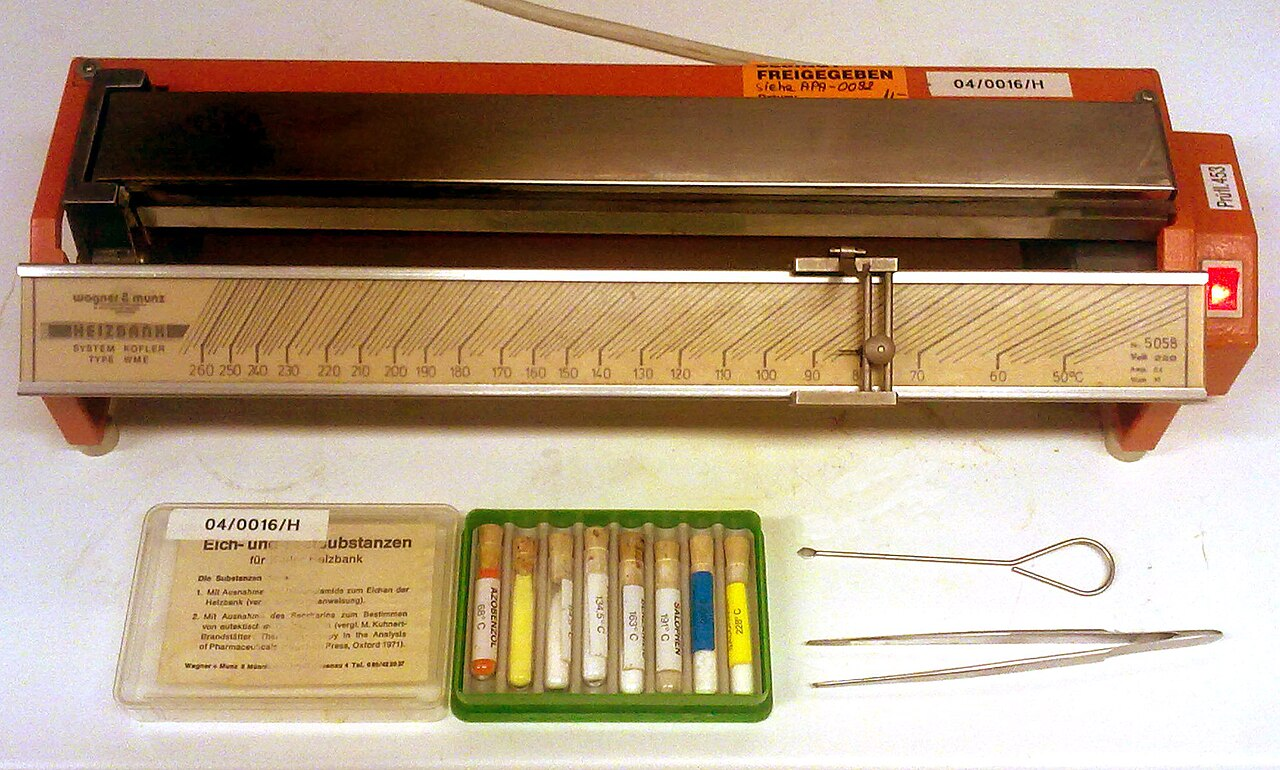
\includegraphics[width=0.62\linewidth]{images/book2/kofler-bench.jpg}

{\small Un banc chauffant (banc Kofler)~: une bande métallique chauffée
à une extrémité, le long de laquelle s'établit un gradient de
température~; le solide, saupoudré sur la bande, fond au-delà d'une
ligne nette, lue sur l'échelle à l'aide du curseur. La boîte contient
des substances de référence de température de fusion connue, qui servent
à l'étalonner. Photo~: HBR, CC BY-SA 3.0, Wikimedia Commons.}
\end{omfigure}

\begin{method}[Mesurer une température de fusion au banc chauffant]\label{met:b1:lab-techniques-1:melting-point}
\begin{enumerate}
  \item Allumer le banc bien à l'avance~: le gradient met du temps à
        s'établir.
  \item L'étalonner avec une substance de référence pure fondant près de
        la valeur attendue, saupoudrée sur la bande~; régler le curseur de
        sorte que l'échelle indique sa température de fusion sur la ligne.
  \item Saupoudrer quelques \omterm{def:b1:crystals-metals:crystal}{cristaux} de l'échantillon sec de l'extrémité
        froide vers l'extrémité chaude~; les pousser d'avant en arrière
        avec la spatule et placer le curseur sur la limite au-delà de
        laquelle le solide fond instantanément.
  \item Lire, recommencer, nettoyer la bande~; prendre la moyenne des
        lectures et indiquer l'incertitude
        (\cref{met:b1:lab-techniques-1:report-result}).
\end{enumerate}
\end{method}

Une espèce cristalline pure fond nettement à sa température de fusion~;
une espèce impure commence à fondre plus bas et fond sur un intervalle
de températures, car l'impureté abaisse la température à laquelle le
solide et le liquide coexistent (la raison, le potentiel chimique d'un
solvant abaissé par un soluté, se trouve dans le volume de deuxième
année). Une température de fusion nettement inférieure à la valeur
tabulée, ou un large intervalle de fusion, révèle donc des impuretés~;
une valeur compatible avec la valeur tabulée, au sens de l'\omterm{def:b1:lab-techniques-1:z-score}{écart
normalisé}, plaide pour la pureté sans la prouver.

\begin{inthelab}[Calibrating the bench]
Les références sont choisies de part et d'autre de la valeur attendue.
L'acétanilide, qui fond à \qty{114.3}{\celsius}, et l'acide benzoïque, à
\qty{122.4}{\celsius}, sont des étalons classiques pour les produits
fondant entre
\qty{110}{\celsius} et \qty{130}{\celsius}~; pour l'aspirine, un étalon
proche de \qty{135}{\celsius} est préférable. L'aspirine elle-même se
décompose en fondant, si bien que sa température de fusion observée
dépend de la vitesse de chauffage~: les tables donnent
\qty{135}{\celsius} pour un chauffage rapide, ce que réalise un banc.
% ledger: mp:acetanilide, mp:benzoic, mp:aspirin
\end{inthelab}

On identifie un liquide, et l'on contrôle sa pureté, par son
\emph{indice de réfraction} $n_D$, rapport de la vitesse de la lumière
dans le vide à sa vitesse dans le liquide, mesuré avec la raie jaune D
du sodium à une température indiquée (en général \qty{20}{\celsius}),
avec quatre décimales. L'eau a pour indice
$n_D = 1.333$, l'éthanol 1.3611 et le cyclohexane 1.4266 à \qty{20}{\celsius}.
L'indice diminue légèrement quand la température augmente~: l'appareil
est donc thermostaté.
% ledger: nD:water, nD:ethanol, nD:cyclohexane

\begin{omfigure}
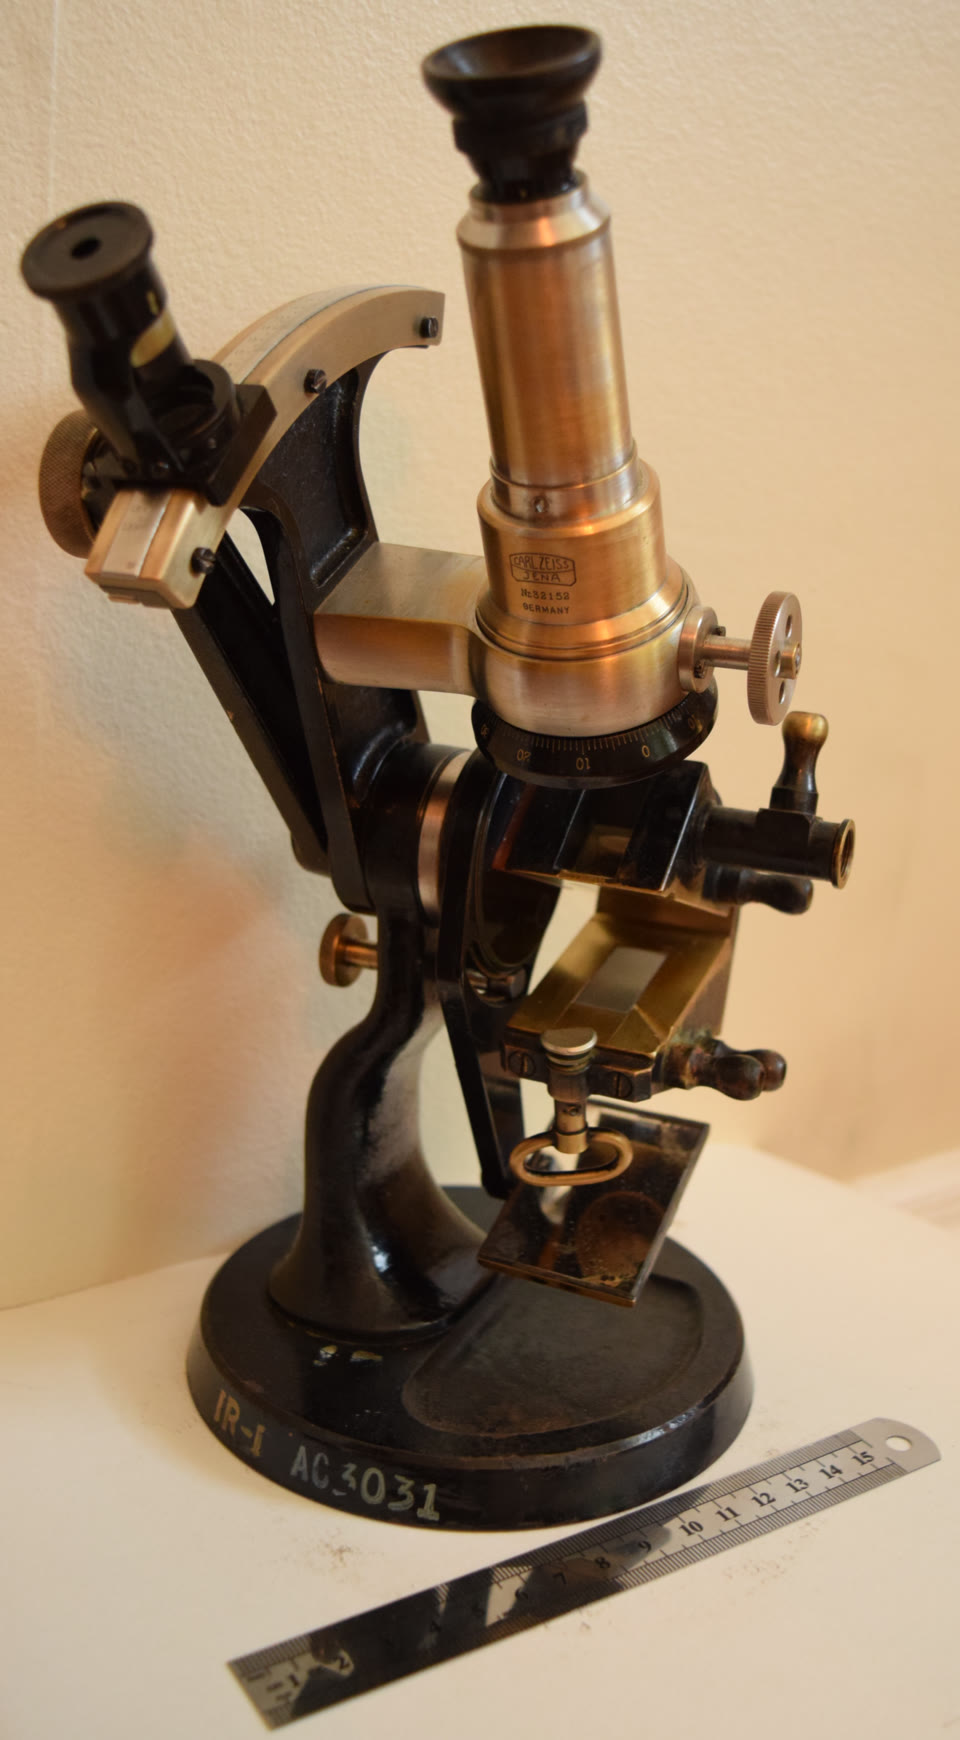
\includegraphics[height=6cm]{images/book2/abbe-refractometer.jpg}

{\small Un réfractomètre d'Abbe~: une goutte de liquide est étalée entre
deux prismes~; l'oculaire montre un champ à moitié clair et à moitié
sombre, et la frontière, placée sur le réticule, donne l'indice de
réfraction sur l'échelle. Photo~: Foreade, CC BY-SA 4.0, Wikimedia
Commons.}
\end{omfigure}

\section{Exercices}

\begin{exercise}[$\star$]\label{exo:b1:lab-techniques-1:1}
Un flacon de propanone porte les pictogrammes GHS02 et GHS07 et les
mentions H225, H319 et H336. Quelle \omterm{def:b1:lab-techniques-1:ghs}{mention d'avertissement} porte-t-il~?
Quelles mentions décrivent un \omterm{def:b1:lab-techniques-1:hazard}{danger} physique, lesquelles un danger
pour la santé~? Citer deux précautions qu'elles imposent.
\end{exercise}

\begin{exercise}[$\star$]\label{exo:b1:lab-techniques-1:2}
\omterm{def:b1:lab-techniques-1:hazard}{Danger} ou \omterm{def:b1:lab-techniques-1:hazard}{risque}~? (a) L'acide sulfurique concentré provoque de graves
brûlures.
(b) Peser \qty{50}{mg} d'une poudre toxique sous la hotte avec des
gants expose peu l'opérateur. (c) Le sodium libère du dihydrogène au
contact de l'eau. (d) Un même solvant est plus dangereux utilisé chaud
dans un bécher ouvert que froid dans un flacon fermé.
\end{exercise}

\begin{exercise}[$\star$]\label{exo:b1:lab-techniques-1:3}
Sur une plaque de CCM, le front de l'éluant se trouve à \qty{6.0}{cm}
au-dessus de la ligne de dépôt~;
l'échantillon donne des taches à \qty{2.1}{cm} et à \qty{4.2}{cm}.
Calculer leurs
$R_f$. Une référence déposée sur la même plaque monte à \qty{4.2}{cm}~:
que peut-on conclure, et que ne peut-on pas conclure~?
\end{exercise}

\begin{exercise}[$\star$]\label{exo:b1:lab-techniques-1:4}
Une burette graduée tous les \qty{0.1}{mL} se lit à une
demi-graduation près. Calculer l'\omterm{def:b1:lab-techniques-1:uncertainty}{incertitude-type} d'une lecture, puis
celle d'un volume délivré, différence de deux lectures.
\end{exercise}

\begin{exercise}[$\star\star$]\label{exo:b1:lab-techniques-1:5}
Cinq pesées d'un même échantillon donnent \qty{0.2512}{g}, \qty{0.2508}{g},
\qty{0.2515}{g}, \qty{0.2510}{g} et \qty{0.2505}{g}. Calculer la moyenne,
l'écart-type expérimental, l'\omterm{def:b1:lab-techniques-1:uncertainty}{incertitude-type} de la moyenne, et
présenter le résultat avec $k = 2$.
\end{exercise}

\begin{exercise}[$\star\star$]\label{exo:b1:lab-techniques-1:6}
Un soluté de \omterm{def:b1:lab-techniques-1:partition-coefficient}{coefficient de partage} $K = 3$ entre un solvant organique
et l'eau est extrait de \qty{50}{mL} d'eau avec \qty{30}{mL} de solvant
au total. Calculer la fraction extraite en une portion, en deux portions
de \qty{15}{mL}, et en trois de \qty{10}{mL}.
\end{exercise}

\begin{exercise}[$\star\star$]\label{exo:b1:lab-techniques-1:7}
Un \omterm{def:b1:titration-methods:titration}{titrage} donne une concentration de \qty{0.1012}{mol/L} avec une
\omterm{def:b1:lab-techniques-1:uncertainty}{incertitude-type} de \qty{0.0006}{mol/L}~; la solution avait été
préparée à \qty{0.1000}{mol/L} avec une \omterm{def:b1:lab-techniques-1:uncertainty}{incertitude-type} de
\qty{0.0002}{mol/L}. Les deux valeurs sont-elles compatibles~? Et si
l'incertitude du \omterm{def:b1:titration-methods:titration}{titrage} avait été de
\qty{0.0004}{mol/L}~?
\end{exercise}

\begin{exercise}[$\star\star$]\label{exo:b1:lab-techniques-1:8}
Les \omterm{def:b1:precipitation:solubility}{solubilités} (valeurs illustratives, en \unit{g} pour \qty{100}{mL})
d'un solide dans trois solvants sont~: solvant P, 1.5 à froid et 2.0 à
ébullition~; solvant Q, 0.3 à froid et 12 à ébullition~; solvant R, 9 à
froid et 25 à ébullition. Quel solvant convient à une \omterm{def:b1:lab-techniques-1:recrystallisation}{recristallisation},
et pourquoi pas les deux autres~? Avec le bon solvant, quelle est la plus
grande fraction de \qty{5.0}{g} du solide que l'on peut récupérer, si
l'on utilise le minimum de solvant bouillant et que l'on refroidit le
mélange~?
\end{exercise}

\begin{exercise}[$\star\star$]\label{exo:b1:lab-techniques-1:9}
Un liquide incolore, thermostaté à \qty{20}{\celsius}, a pour indice
$n_D = 1.3612$. Lequel de l'eau, de l'éthanol et du cyclohexane peut-il
être~? Pourquoi précise-t-on la température~? Que suggérerait une valeur
de 1.350~?
\end{exercise}

\begin{exercise}[$\star\star\star$]\label{exo:b1:lab-techniques-1:10}
Avec les données de l'\cref{exo:b1:lab-techniques-1:6}, montrer que, si
finement que l'on divise les \qty{30}{mL} de solvant, on ne peut
extraire au plus qu'une fraction
$1 - \mathrm{e}^{-KV/V_a}$ du soluté, et la calculer.
Combien de portions faut-il pour atteindre \qty{99}{\percent} de cette
limite~?
\end{exercise}

\begin{exercise}[$\star\star\star$]\label{exo:b1:lab-techniques-1:11}
Une grandeur est comprise entre $x_0 - a$ et $x_0 + a$, les valeurs
proches de
$x_0$ étant plus probables~: sa densité est triangulaire,
$(a - |x - x_0|)/a^2$. Vérifier qu'elle est normalisée et montrer que
son \omterm{def:b1:lab-techniques-1:uncertainty}{incertitude-type} vaut
$a/\sqrt6$. Comparer avec le cas rectangulaire.
\end{exercise}

\begin{exercise}[$\star\star\star$]\label{exo:b1:lab-techniques-1:12}
On prépare une solution étalon en dissolvant l'échantillon de
l'\cref{exo:b1:lab-techniques-1:5} (masse molaire \qty{204.2}{g/mol},
d'incertitude négligeable) dans une fiole jaugée de \qty{100.00}{mL}
dont le volume a une \omterm{def:b1:lab-techniques-1:uncertainty}{incertitude-type} de \qty{0.06}{mL}. Calculer la
concentration et ses \omterm{def:b1:lab-techniques-1:uncertainty}{incertitudes relative} et élargie. Quelle source
domine~?
\end{exercise}

\section{Problème~: purifier l'aspirine}

\begin{problem}[{Problème du week-end --- les dangers d'une synthèse, la
recristallisation de l'aspirine brute et son rendement, une température
de fusion avec ses incertitudes de type A et de type B, et l'écart
normalisé à la valeur tabulée}]
\label{pb:b1:lab-techniques-1:1}
Un étudiant prépare de l'aspirine en chauffant \qty{2.00}{g} d'acide
salicylique avec un excès d'anhydride éthanoïque, puis recristallise le
produit brut. Masses molaires (\unit{g/mol})~: acide salicylique
\ce{C7H6O3} 138.0, aspirine
\ce{C9H8O4} 180.0, anhydride éthanoïque \ce{C4H6O3} 102.0.
Étiquettes~: acide salicylique GHS05, GHS07, H302, H318~; anhydride
éthanoïque GHS02, GHS05, GHS06, GHS07, H226, H302, H314, H332~;
aspirine GHS07, H302. \omterm{def:b1:precipitation:solubility}{Solubilité} de l'aspirine dans l'eau~:
\qty{3.3}{g/L} à \qty{25}{\celsius}. Température de fusion tabulée de
l'aspirine (chauffage rapide)~: \qty{135}{\celsius}.
% ledger: ghs:salicylic, ghs:acetic-anhydride, ghs:aspirin, sol:aspirin-25,
% mp:aspirin, hstat:H318, hstat:H226, hstat:H314, hstat:H302

\medskip
\noindent\textbf{Partie I --- Les \omterm{def:b1:lab-techniques-1:hazard}{dangers}.}
\begin{enumerate}
  \item Que signifie chaque pictogramme de l'étiquette de l'anhydride
        éthanoïque~?
  \item Quelle \omterm{def:b1:lab-techniques-1:ghs}{mention d'avertissement} l'étiquette de l'acide
        salicylique porte-t-elle~? Et celle de l'aspirine~?
  \item L'anhydride éthanoïque présente les \omterm{def:b1:lab-techniques-1:hazard}{dangers} les plus graves.
        Expliquer comment le \omterm{def:b1:lab-techniques-1:hazard}{risque} lié à la manipulation de
        \qty{5}{mL} de ce réactif peut néanmoins être rendu faible.
  \item Lesquelles des mentions de l'anhydride imposent lunettes et
        gants, et lesquelles la hotte et l'absence de flamme~?
  \item Que fait-on immédiatement si une goutte d'anhydride atteint un
        œil~?
  \item Le filtrat de la \omterm{def:b1:lab-techniques-1:recrystallisation}{recristallisation} contient de l'acide
        éthanoïque et un peu d'éthanol dans l'eau. Où va-t-il~?
\end{enumerate}

\noindent\textbf{Partie II --- Synthèse et \omterm{def:b1:lab-techniques-1:recrystallisation}{recristallisation}.}
\begin{enumerate}[resume]
  \item Écrire l'équation de la synthèse, avec l'acide éthanoïque
        \ce{C2H4O2} comme sous-produit, et vérifier qu'elle est
        équilibrée.
  \item Calculer la quantité de matière d'acide salicylique et la masse
        maximale d'aspirine.
  \item Le produit brut sec pèse \qty{2.41}{g}. Pourquoi ne peut-on pas
        se passer de la \omterm{def:b1:lab-techniques-1:recrystallisation}{recristallisation}, bien que cela représente
        \qty{92}{\percent} du maximum~?
  \item L'aspirine est recristallisée dans un peu d'éthanol complété par
        de l'eau chaude. Pourquoi la propriété déterminante est-elle la
        \omterm{def:b1:precipitation:solubility}{solubilité} dans l'eau à \qty{25}{\celsius}, comparée à celle près
        de l'ébullition~?
  \item Pourquoi dissout-on le solide brut dans le minimum de solvant
        chaud~?
  \item Pourquoi refroidit-on la solution lentement, puis dans la glace~?
  \item \qty{40}{mL} de filtrat à \qty{25}{\celsius} quittent
        l'entonnoir, puis \qty{5}{mL} d'eau de lavage. Estimer la masse
        d'aspirine perdue avec eux.
  \item Le produit pur et sec pèse \qty{1.95}{g}. Calculer le \omterm{def:b1:extent-q-and-k:fractional-extent}{rendement}.
\end{enumerate}

\noindent\textbf{Partie III --- La température de fusion.}
\begin{enumerate}[resume]
  \item Six lectures sur le banc, étalonné juste avant, donnent 134, 135,
        133, 135, 134 et \qty{136}{\celsius}. Calculer la moyenne.
  \item Calculer l'écart-type expérimental.
  \item En déduire l'\omterm{def:b1:lab-techniques-1:uncertainty}{incertitude-type} de type A de la moyenne.
  \item Chaque lecture est faite au degré près. Calculer l'incertitude
        de lecture de type B.
  \item L'étalonnage du banc est garanti à
        $\pm\qty{1}{\celsius}$ près. Calculer l'incertitude de type B
        correspondante, puis l'\omterm{def:b1:lab-techniques-1:uncertainty}{incertitude-type} composée.
  \item Présenter la température de fusion avec son \omterm{def:b1:lab-techniques-1:uncertainty}{incertitude élargie}
        ($k = 2$).
  \item Le produit brut d'un camarade fond entre 120 et
        \qty{128}{\celsius}. Qu'est-ce que cela indique~?
\end{enumerate}

\noindent\textbf{Partie IV --- Comparaison avec la référence.}
\begin{enumerate}[resume]
  \item La valeur tabulée est donnée à l'unité. Quelle \omterm{def:b1:lab-techniques-1:uncertainty}{incertitude-type}
        cela implique-t-il~?
  \item Sur une plaque de CCM (front à \qty{6.0}{cm}), le produit brut
        présente des taches à \qty{2.3}{cm} et à \qty{3.3}{cm}, l'acide
        salicylique une tache à \qty{2.3}{cm}, le produit recristallisé
        une tache à \qty{3.3}{cm}. Calculer les valeurs de $R_f$ et
        conclure.
  \item Pourquoi la température de fusion de l'aspirine dépend-elle de la
        vitesse de chauffage~?
  \item Calculer l'\omterm{def:b1:lab-techniques-1:z-score}{écart normalisé} $z$ entre la température de fusion
        mesurée et la température tabulée, et dire si elles sont
        compatibles.
\end{enumerate}
\end{problem}
